\chapter{重定向后的交互强化}

\section{直接使用重定向结果的缺陷}
尽管本方法重定向结果已经达到较高精度和平滑度，但在实际应用中仍存在不足之处：

首先，现实生活中，人在抓取物体的过程中，通常会根据物体来预测大致抓取力，而在本方法的灵巧手抓取物体的过程中，
抓取力在未接触物体时与加速度相关，在与物体接触时，则受到电机最大力矩和物体表面性质影响。
而在此过程中有可能在接触时，就因加速度过大，导致灵巧手的抓取力过大，进而损坏物体。
而一直让灵巧手保持低速运行又显然是一个过于保守的策略。
因此，我们认为在对一个物体进行抓取前，应该先大致预测抓取力，
并在抓取前调整灵巧手电机速度，使得抓取力与预测值一致。
具体的，我们认为可以通过视觉语言模型来预测抓取力，并在即将抓取时，将灵巧手电机速度调整以匹配预测抓取力。

其次，本方法仅根据人手位置生成灵巧手角度，没有考虑灵巧手手指与目标之间的距离等交互信息。
特别是涉及物体表面性质的信息，例如对于易碎或者弹性物体，抓取力可能需要根据物体的材质进行调整，而不仅仅是根据人手的动作来确定。
如果人手在遥操作的过程中，对应灵巧手动作将要穿透物体表面，那么此时就需要根据触觉信息或者关节力矩信息进行修正，
避免抓取动作破坏物体。

最新研究将机器学习与多变量控制（MPC）相结合，通过建立关节角度与接触力之间的映射关系，实现了力预测与调控功能。例如，徐等人[27]采用GelSight触觉反
馈系统进行实时调节，史等人\cite{vulinImprovedLearningRobot2021}将基于高斯过程的状态与力关系建模方法整合到安全约束型MPC框架中，田
等人\cite{huPhysicalInteractionReconstructing2022}则将深度强化学习与力反馈技术相结合，实现多指自适应抓取控制。尽管这些方法能提供在线力控制
与预测能力，但多数仍依赖离线训练模式，或缺乏对目标力场的智能感知能力及任务特定适应性。

在本工作中，我们尝试将基于VLM的目标抓取力预测与基于力矩反馈的强化学习相结合，以实现在线抓取力的预测和控制。

\section{基于VLM的目标抓取力预测}
\subsection{VLM简述}
VLM全称视觉语言模型，是一种结合了视觉和语言理解能力的人工智能模型。通过对图像和文本数据的联合训练，VLM能够从视觉输入中提取语义信息，
并将其与语言描述进行关联，从而实现对图像内容的理解和生成相关文本的能力。

\subsection{大模型结合的目标抓取力预测}
首先人手抓取物体中涉及几个物理量，譬如在抓取水瓶时，简化后的物理过程可以用以下式子表示：
\begin{equation}
    F_{grasp} \geq \frac{m(g + a)}{n \cdot \mu}
\end{equation}
其中：
\begin{itemize}
    \item $ m $：水瓶的总质量。
    \item $ g $：重力加速度。
    \item $ a $：机器人手臂运动时的垂直加速度。
    \item $ n $：接触面的数量。
    \item $ \mu $：摩擦系数。
\end{itemize}
要直接实时测量这些物理量显然不现实，且没有实际应用价值。在交互过程中，我们仅需要给灵巧手关节设置一个大致的扭矩即可，而这个扭矩决定抓取力矩大小。
因此我们想到借助大模型输入一帧图像或者一句话，来预测一个大致的抓取力矩。我们会给予大模型物体类别提示词，希望模型能够根据提示词或图像生成一个安全的抓取力矩以防止损坏物体。
相较于传统基于传感器或启发式力阈值判定的方法，该方案充分利用大型模型的丰富知识库，直接将物体类别映射至所需作用力。例如当识别物体为“水瓶”时，模型可推断推荐
手指整体抓取力约为10N，为后续自适应调整提供初始参考依据。或者在此场景下，VLM推断的主要优势在于能够基于知识驱动的洞察力，对目标力进行先验估计。
在复杂的多目标环境中，手动校准或固定阈值常常难以在把握稳定性与物体安全性之间取得平衡。通过运用语义感知和先验知识， 大模型可以根据视觉输入或者语言描述生成合理的目标力，从而有效启动自适应力控制过程。

当然，VLM的预测结果往往与实际抓取力有偏差，因此灵巧手关节的扭矩需要在其与物体交互后进一步调整。

\section{基于力矩反馈的强化学习}
\subsection{强化学习简述}
强化学习是机器学习的一种，与监督学习和无监督学习不同，强化学习通过与环境的交互来学习最优策略。智能体在每个时间步观察环境状态，采取动作，并根据环境反馈的奖励信号调整其行为策略，以最大化累积奖励。
而在机器人控制领域，强化学习已被广泛应用于复杂任务的学习和优化，如机械臂操作、路径规划等。
\subsection{力矩反馈的自适应关节角度调整}
近年来，深度强化学习技术已成为控制复杂动态系统的重要方法，尤其在高维精细操作领域表现突出
\cite{sheLearningHighDOFReachingandgrasping2022}\cite{christenDgraspPhysicallyPlausible2022}。
这类方法通常依赖人类示范\cite{rajeswaranLearningComplexDexterous2017}，或假定对物体姿态具有精确认知。

从预抓取到目标功能性抓取的运动规划并不容易，与夹爪开闭的抓取动作不同，五指灵巧手抓取物体时，需要五指以合适的姿态和力度进行协同，才能实现稳定的抓取。
同时，灵巧手与物体交互的过程中会产生遮挡效应，如果根据视觉信息判断抓取情况会十分困难。
基于人类的操作演示，可以让灵巧手粗略模仿人手动作，但在与物体交互后就应该根据反馈信息进行调整。
当前许多研究基于夹爪式抓取器的力反馈进行探索\cite{RL28}，但将这种技术推广到五指灵巧手面临重大挑战。
狭义的触觉传感器即置于手指表面的电子元件，用于测量触点的压力或者切向力，但成本高昂。故可以在重定向的基础上，通过关节扭矩指导手部抓取动作。同时关节扭矩反馈有助于定位
物体、感知其几何结构并提供顺应性接触力。

因此，我们认为在抓取过程中，基于关节力矩的反馈信息进行自适应调整是一个更为可靠的方案，而且考虑到使用关节力矩进行触觉的模拟以实现低成本的力反馈。

在本节中，我们通过构建一个强化学习模型，将关节扭矩反馈被视作马尔可夫决策过程中的状态变量之一，这使得机器人能够在姿态不确定性条件下通过试错学习抓取技能。
为方便表述，本节我们定义重定向的结果为预抓取角度，交互强化模块输出的角度为辅助关节角度，最终输出为输出关节角度。
\subsection{师生策略}
在强化学习过程中，我们采用了师生策略的架构设计。如图\ref{fig:TSnet}所示，在训练的过程中，我们会训练两个策略，教师策略拥有更多的信息用来辅助训练，学生策略则被用于实际预测和控制。
首先我们会用更多的信息来训练教师策略，然后通过教师策略输出的参数作为学生策略的参考，进行学生策略的训练。
在此之后我们会将教师策略提炼为学生策略，在学生策略训练，我们会限制学生策略的输入信息，使其只能使用教师策略输入的一部分信息进行训练。
这样做的目的是为了让学生策略能够在实际应用中使用更少的信息进行预测和控制。

\begin{figure}
    \centering
    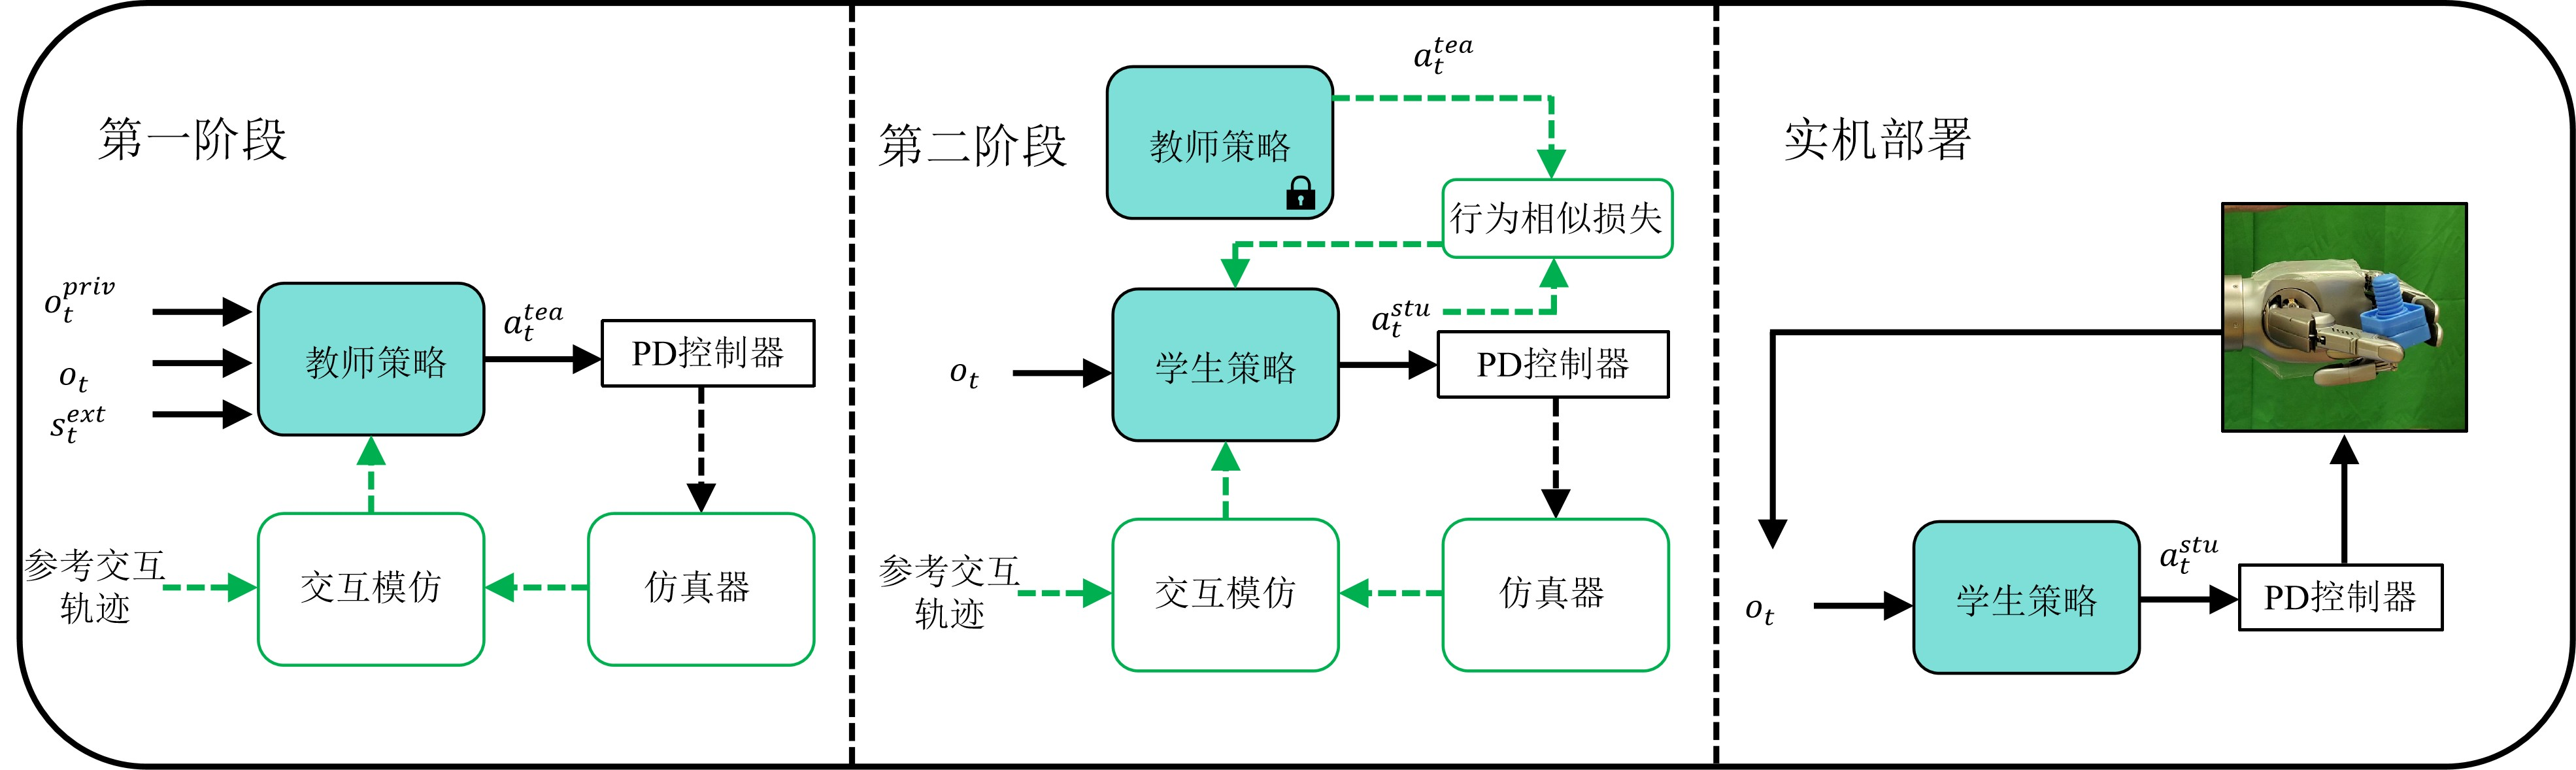
\includegraphics[width=0.95\textwidth]{figure/TSnet.jpg}
    \caption{师生策略结构图。}
    \label{fig:TSnet}
\end{figure}
\subsection{动作和状态空间}
动作空间包含17个控制量，分别对应灵巧手的17个关节的目标角度，以及控制手部底座平移和旋转的关节。
状态空间则包含当前手指关节的扭矩、角度、手部姿态以及物体姿态等信息。
\begin{table}[h]
\centering
\begin{tabular}{cccc}
\toprule
观察量 & 维度 & 教师策略 & 学生策略\\
\midrule
输入指定扭矩 & 17 & \checkmark & \checkmark \\
当前手部关节扭矩 & 17 & \checkmark & \checkmark \\
当前手部关节角度 & 17 & \checkmark &  \checkmark \\
当前手部6维姿态 & 6 & \checkmark & \checkmark \\
当前物体姿态 & 6 & \checkmark & $\times$ \\
\bottomrule
\end{tabular}
\caption{观察量列表}
\label{tab:grasp_parameters}
\end{table}


\subsection{奖励机制}
在我们的操作任务中，由于物体初始位置存在不确定性，灵巧手需要通过触觉感知物体的真实位置。
在此过程中，手部与物体之间的接触碰撞可能导致物体进一步位移。而合格的抓取动作应该能够尽量减少物理位移，
或者在接触后迅速调整手部姿态以适应物体的位移，从而实现稳定的抓取。
由于在实际交互算法中，操作时间主要消耗在寻找合适的抓取姿态上，但此部分操作可以由遥操作完成，故奖励函数可以不用考虑操作时间。
因此，我们设计了一个综合考虑接触质量、抓取稳定性的奖励函数。整体奖励函数为：
\begin{equation}
r = r_{diff} + r_{obj} + r_{rel} + r_{cont} + r_{regt}.
\end{equation}
下面简单介绍一下每个奖励项的含义：
重定向差异奖励$r_{diff}$用于鼓励教师策略输出的关节角度与重定向结果的关节角度接近，以帮助教师策略学习重定向结果的行为模式。
但此项不能过于强调，否则会导致教师策略过度依赖重定向结果，完全忽略交互信息。在实际使用时可以根据训练轮数逐渐降低该项的权重。
而这一项用在学生策略中则是为了让学生策略能够学习教师策略的行为模式，从而更好地模仿教师策略的行为。也是不能过度强调，否则会导致学生策略过度依赖教师策略，完全忽略交互信息。
输出关节角度与参考角度的差异越小，则奖励越大。

物体偏移奖励$r_{obj}$用于奖励物体位移较小的抓取动作，以确保抓取的稳定性。计算前首先会记录物体在交互前的初始位姿，然后在抓取物体时候记录物体的当前位姿，并计算物体位移和旋转。
物体偏移越大，则奖励越小。

相对运动奖励$r_{rel}$用于奖励手指与物体之间相对运动较小的抓取动作，以减少物体在抓取过程中的滑动。
理想的抓取应该是不会产生滑动的，此项奖励函数计算手部与物体之间的相对运动。将手掌和物体抽象为两个点，在抓取动作执行后，若发生滑动次数越多，则奖励越小。

接触奖励$r_{cont}$用于奖励手指与物体之间接触良好的抓取动作，以确保抓取的可靠性。在大部分物体抓取过程中，手指应该尽量都接触物体，
故此项奖励函数计算手指与物体之间的接触情况，接触点越多，则奖励越大。当然接触情况也和物体大小有关，故本奖励函数在计算较小物体的接触奖励时可能会有无法提高奖励的问题。
正则化项$r_{regt}$用于防止策略过拟合，提高策略的泛化能力。
该项主要对训练的策略进行正则化约束，防止过拟合。

\subsection{交互强化与重定向结果的融合}
整个多指手部由6自由度手部基座及每个关节配备的执行器共同控制。手部基座通过全局调整整个手部的姿态
与位移，使其能够到达物体的可行接近方向与距离；而每个关节的执行器则通过局部控制关节角度，使多根手
指接触物体的对应功能部位。另外考虑到交互强化和预抓取角度应该存在一个可调的参数，以控制操作者操作的自主性，且由于从预抓取到目标抓取过程中手指与物体之间间隙非线性，
完全依赖交互强化会导致优化失败，因此我们将交互强化模块看做是一个辅助模块，设置了一个辅助强度参数，控制其对重定向结果的影响程度。我们为每个
关节采用局部线性轨迹控制方案。该轨迹以预抓取抓取角度$J_0$、辅助关节角度$J_g$以及参数$h$为输入参数，输出关节角度$J$，过程如下：
$$J = h(J_g - J_0) + J_0, h \in [0, 1].$$

上式中，h表示辅助强度参数，取值范围在0到1之间，取值越小，对交互辅助越弱，取值越大，对交互辅助越强。
当h=0时，关节角度$J$与预抓取抓取角度$J_0$相同，当h=1时，关节角度$J$与辅助关节角度$J_g$相同。